\section{Introduction}

Large model size and overparameterization in deep learning are known to improve generalization performance \cite{neyshabur2017geometry}, and, state-of-the-art deep neural networks (DNNs) can be outrageously large. However, such large models are not suitable for certain important application domains, such as mobile computing \cite{tan2019mnasnet,sandler2018mobilenetv2}. Pruning algorithms aim to address the challenge of building lightweight DNNs for such domains. While there are several pruning methods, their common goal is to compress large DNN models by removing weak connections/weights with minimal decline in accuracy. Here, a key empirical phenomenon is that {\em{it is often better to train and prune a large model rather than training a small model from scratch}}. Unfortunately, the mechanisms behind this phenomenon are poorly understood especially for practical gradient-based algorithms. This paper sheds light on this by answering: {\em{What are the optimization and generalization dynamics of pruning overparameterized models? Does gradient descent naturally select the good weights?}} 


% for building good lightweight models 
%An important drawback of deep neural networks (DNN) is that they are computationally demanding 

%A core challenge in machine learning stems from {\em{limited hardware budgets}}. 
% with substantial computation cost e.g.~OpenAI's latest language model has 175 billion parameters and would cost \$4.6 million to train \cite{gpt3}
%State-of-the-art deep neural networks (DNN) can be outrageously large. At the other end of the spectrum, while mobile platforms such as smartphones and unmanned aerial vehicles provide key application domains for \ML, they require lightweight models that are energy and storage efficient during inference  
\vp
\noindent{\bf{Contributions:}} %Our core contribution is a thorough
%theoretical
We analytically study the performance of popular pruning strategies. First, we analyze linear models, and then, generalize the results to nonlinear feature maps. Through extensive simulations, we show that our analytical findings predict similar behaviors in more complex settings.  

%\textbf{(a)}
\noindent\textbf{(a)} {\bf{Distributional characterization (DC):}} The key innovation facilitating our results is a theoretical characterization of the distribution of the solution of overparameterized least-squares. This DC enables us to accurately answer {\em{``what happens to the accuracy if X\% of the weights are pruned?''}}.

\noindent\textbf{(b)} {\bf{Benefits of overparameterization:}} Using DC, we 
%exactly
 %and provably 
{obtain rigorous precise characterizations of  the pruning performance in linear problems. Furthermore, we use, so called ``linear gaussian equivalences", to obtain sharp analytic predictions for nonlinear maps, which we verify via extensive numerical simulations.}
%for pruning strategies and verify our predictions for nonlinear maps via establishing linear equivalences. 
 By training models of growing size and compressing them to fixed sparsity, we identify a novel double descent behavior, where the risk of the pruned model is 
 %often
{consistently} minimized in the overparameterized regime. Using our theory, we uncover rather surprising scenarios where pruning an overparameterized model is provably better than training a small model with the exact information of optimal nonzero locations. 
%\som{neural net does not keep the optimal locations}
%\ct{need to be careful here}

\noindent\textbf{(c)} {\bf{Benefits of retraining:}} An important aspect of pruning is retraining the model using the favorable nonzero locations identified during the initial training. We show that retraining can actually hurt the performance when features are uncorrelated. However, it becomes critical as correlations increase. Importantly, we devise the DC of the {\em{train$\rightarrow$prune$\rightarrow$retrain process}} (see Figs.~\ref{figRF} and \ref{figRF2} and the discussion around Def.~\ref{RT_def} for details), and, we demonstrate that it correctly captures the pruning performance of random features  that are known to be good proxies for understanding DNN behavior \cite{jacot2018neural}. 

{We anticipate that our techniques towards establishing the DC of the overparameterized problems might be useful, beyond the context of pruning, in other statistical inference tasks that require careful distributional studies.}
%Of general interest, we emphasize that our high-dimensional analysis of the complex procedures like pruning are entirely novel and we anticipate that our techniques can help address other interesting statistical learning tasks which require a careful distributional characterization.% This also reveals different pruning double-descents.
% are known to be a good proxy to understand the pruning in neural nets.



\begin{figure}[t!]
\centering
	\begin{tikzpicture}
	\node at (0,0) {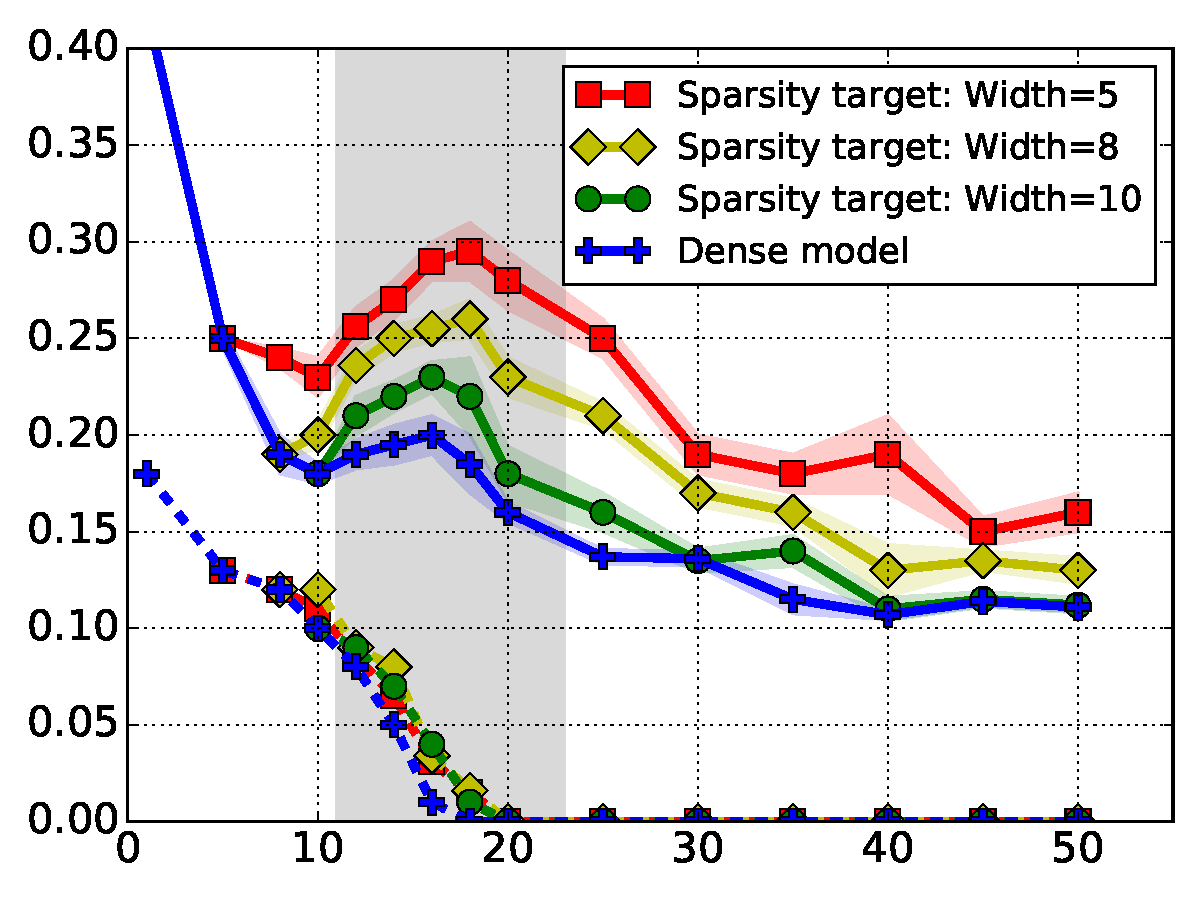
\includegraphics[scale=0.33]{figs/CIFAR10_New_DD}};
	\node at (-3.5,0) [rotate=90,scale=1.]{Training / Test Error};
	\node at (0,-2.6) [scale=.9]{Width Parameter (\# of filters $k$)};%Each bar in the figure shows the correlations' geometric mean of datasets in this group when training to corresponding non-zero level. 
%	\node (A) at (0, 0) {A};
%	\node (B) at (1, 1) {B};
%	\draw [->] (A) edge (B) 
	\end{tikzpicture}
	\vspace{-10pt}
	\caption{\small{We train sparse ResNet-20 models on the CIFAR-10 dataset with varying width (i.e. number of filters) and sparsity targets. The width parameter controls the overall model size. The solid (resp. dashed) lines are test (resp. training) errors. The blue line corresponds to training of a dense model with width-$k$. The other three curves correspond to sparsity targets $s\in\{5,8,10\}$, for which a dense model of width-$k$ is first pruned to achieve the exact same number of nonzeros as a dense model of width-$s$ and then retrained over the identified nonzero pattern. Surprisingly, all curves interpolate (achieve zero training error) around the same width parameter despite varying sparsity. The best test error is always achieved in the overparameterized regime (large width). Test error curves have two local minima which uncovers a novel double descent phenomena for pruning. {The shaded region highlights the transition to zero training error, where the test error peaks.}}}
	%We train and prune ResNet-20 models on the CIFAR-10 dataset with varying filter numbers (which modifies the total number of parameters) and sparsity targets. Solid and dotted lines are test and training error respectively. The dense line shows training results with $k$ filters. Correspondingly, the other two lines prune dense model to sparse ResNet-20 and make sure they have the same number of non-zero parameters as dense $s$-filter ResNet-20. From red and green curves, training and test error decrease with model size, implying that training and pruning a larger model preforms better than training small model.  Secondly, a novel double descent phenomena appears when training with sparse models .
	\label{figNN}\vspace{-15pt}
\end{figure}

%\somm{it might be good to move the sentence from appendix to the main body that this train error is actually the retrain error!}
\subsection{Prior Art}
%, as well as, optimization dynamics
This work relates to the literature on model compression and overparameterization in deep learning. 
%For analysis, we also use tools related to high-dimensional statistics \cite{thrampoulidis2015regularized,OymLAS,thrampoulidis2018precise,hastie2019surprises}. 
% by the problem structure
%Recent works use \emph{magnitude-based} \cite{han2015learning,frankle2019lottery,franklestabilizing} and \emph{Jacobian-based} \cite{shunshi2019one} pruning criteria, which are shown to achieve stellar performance. 

%There are various saliency-based approaches \cite{hassibi1993second,hassibi1994optimal,lecun1990optimal,dong2017learning} for neural net pruning to select .
\vs\noindent {\bf{Neural network pruning:}} Large model sizes in deep learning have led to a substantial interest in model pruning/quantization \cite{han2015deep,hassibi1993second,lecun1990optimal}. DNN pruning has a diverse literature with various architectural, algorithmic, and hardware considerations \cite{sze2017efficient,han2015learning}. The pruning algorithms can be applied before, during, or after training a dense model \cite{lee2018snip,wang2020picking,jin2016training,oymak2018learning} and in this work we focus on after training. Related to over-parameterizarion, \cite{frankle2018lottery} shows that a large DNN contains a small subset of favorable weights (for pruning), which can achieve similar performance to the original network when trained with the same initialization. \cite{zhou2019deconstructing,malach2020proving,pensia2020optimal} demonstrate that there are subsets with good test performance even without any training and provide theoretical guarantees. However, these works do not answer why practical gradient-based algorithms lead to good pruning outcomes. {Closer to us, \cite{li2020exploring} derives formulas for predicting the pruning performance of over-parameterized least-squares without proofs. In contrast, we provide provable guarantees, and, also obtain DC for more complex problems with general design matrices and nonlinearities.}

%For example, \cite{lee2018snip,wang2020picking} \ct{I don't understand this sentence}prune the network before training by the connection sensitivity and gradient flow, respectively. Furthermore, \cite{aghasi2017net,oymak2018learning,jin2016training} use $\ell_1$-penalization pruning strategies, for which they provide provable performance guarantees. 

\begin{figure}[t!]
\centering
	\begin{tikzpicture}
	\node at (0,0) {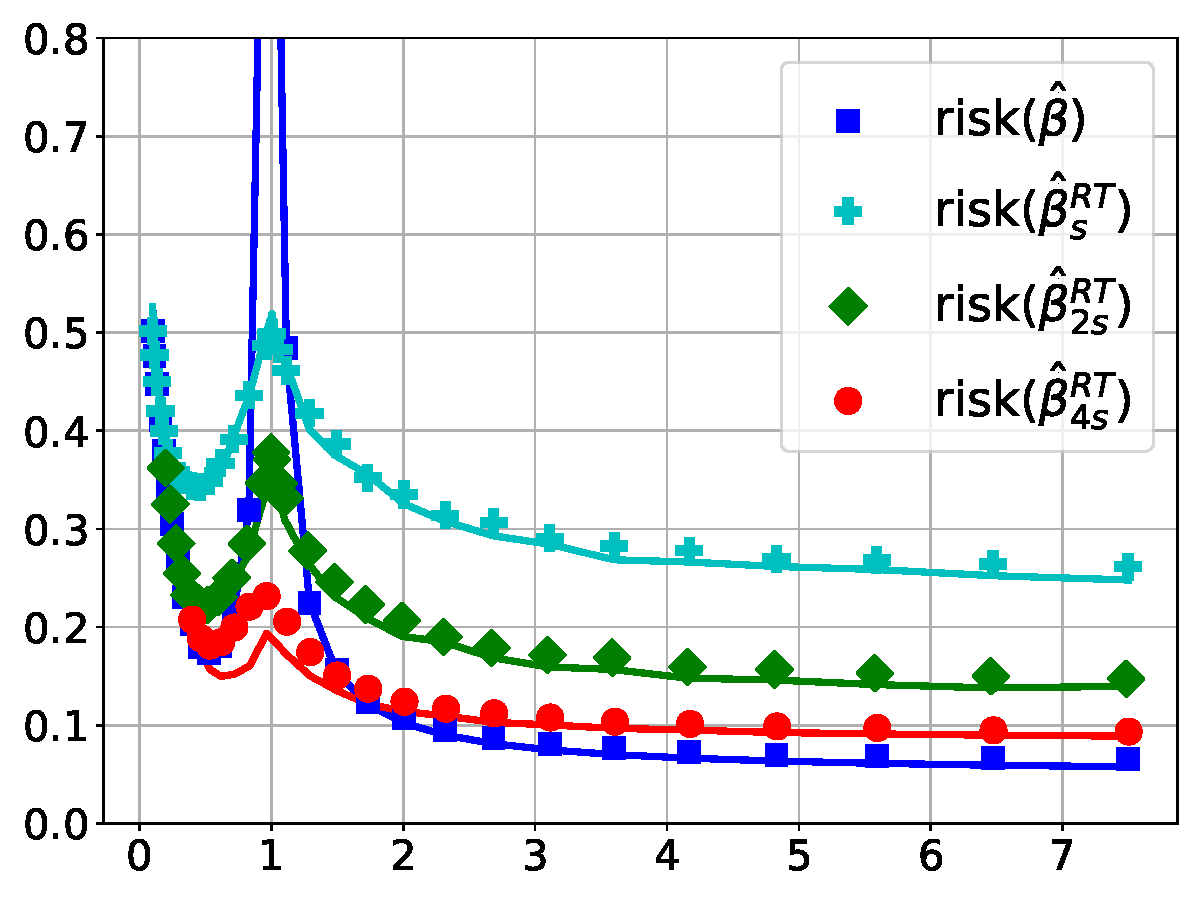
\includegraphics[scale=0.33]{figs2/RF_COMBINED_80_n200_p1500}};
	\node at (-3.5,0) [rotate=90,scale=1.]{Test Risk};
	\node at (0,-2.6) [scale=.9]{Overparameterization ($p/n$)};%Each bar in the figure shows the correlations' geometric mean of datasets in this group when training to corresponding non-zero level. 
	\end{tikzpicture}
	\vspace{-10pt}
	\caption{\small{Random feature regression (RFR) with ReLU feature-map $\phi(\ab)=\text{ReLU}(\Rb\ab)$. Here $\Rb$ has i.i.d.~standard normal entries corresponding to the input layer of a shallow neural net and we regress the output layer. Solid lines follow from our distributional characterization and the markers are obtained by solving random feature regression, which exhibit a good match. The blue line is the performance of usual RFR with growing number of features $p$. The other lines are obtained by solving RFR with $p$ features and pruning and retraining the solution to fixed sparsity levels ($s,2s,4s$) with $s/n=0.1$. Importantly, the risks of the retrained models exhibit double descent and are minimized when $p\gg n$ despite fixed model size / sparsity. The slight mismatch of the red curve/markers is explained in Fig.~\ref{figRF2}.}}%,mei2019generalization
	\cmt{We emphasize that RFR is a well-recognized proxy for the DNN regression due to the equivalence between kernels and wide DNNs \cite{jacot2018neural}.}
	\label{figRF}\vspace{-15pt}
\end{figure}
\cmt{The green line prunes the resulting coefficients to find a sparse model with fixed sparsity $s/n=0.1$. The red line resolves RFR using the features identified after pruning. All lines exhibit double descent at $n=p$.}
%oymak2019overparameterized
\noindent {\bf{Benefits of overparameterization:}} Studies on the optimization and generalization properties of DNNs demonstrate that overparameterization acts as a catalyst for learning. \cite{arora2018optimization,neyshabur2014search,gunasekar2017implicit,ji2018risk} argue that gradient-based algorithms are implicitly biased towards certain favorable solutions (even without  explicit regularization) to explain benign overfitting \cite{bartlett2020benign,oymak2020towards,du2019gradient,chizat2019lazy,belkin2018understand,belkin2019does,tsigler2020benign,liang2018just,mei2019generalization,ju2020overfitting}. More recently, these studies have led to interesting connections between kernels and DNNs and a flurry of theoretical developments. Closest to us, \cite{nakkiran2019deep,belkin2019two,belkin2019reconciling} uncover a double-descent phenomenon: the test risk has two minima as a function of model size. One minimum occurs in the classical underparameterized regime whereas the other minimum occurs when the model is overparameterized and the latter risk can in fact be better than former. Closer to our theory, \cite{derezinski2019exact,hastie2019surprises,montanari2019generalization,deng2019model,kini2020analytic,liang2020precise,salehi2020performance,ju2020overfitting} characterize the asymptotic performance of overparameterized learning problems. However these works are limited to characterizing the test error of regular (dense) training. In contrast, we use distributional characterization (DC) to capture the performance of more challenging pruning strategies and we uncover novel double descent phenomena (see Fig.~\ref{figNN}).

%A related line of work connects the benefits of overparameterization to the double descent phenomena \cite{nakkiran2019deep,belkin2019two,belkin2019reconciling,hastie2019surprises,deng2019model}. 


\cmt{For linear models, implicit bias phenomena have been studied for various loss functions and algorithms (e.g.~logistic loss converging to max-margin solution on separable data) \cite{ji2018risk,soudry2018implicit,nacson2019stochastic}. Follow-up works show that such results continue to hold for nonlinear problems \cite{gunasekar2017implicit,oymak2019overparameterized,azizan2018stochastic}. More recently, this line of works has further motivated the study of generalization/optimization guarantees for deep networks and their connections to random features \cite{du2019gradient,allen2019convergence,chizat2019lazy,belkin2018understand,belkin2019does,liang2018just,mei2019generalization}.}



